%========================================================================================
%  TESI TRIENNALE — Lorenzo Caivano
%  File principale: compila SEMPRE questo file (VS Code + LaTeX Workshop lo fa da solo).
%  Il testo vero sta nei file della cartella Capitoli/ — qui ci sono solo impostazioni,
%  frontespizio e l'elenco dei capitoli.
%========================================================================================

\PassOptionsToPackage{italian}{babel}   % il template carica babel senza lingua: gliela passiamo qui
\documentclass[12pt, oneside]{MastersDoctoralThesis}
% 12pt      = dimensione del font
% oneside   = stampa solo fronte (margini uguali a destra e sinistra)
% (la riga \PassOptionsToPackage sopra mette "Indice", "Capitolo", "Figura", "Bibliografia" in italiano)

\usepackage[utf8]{inputenc}   % lettere accentate scritte direttamente (è, à, ...)
\usepackage[T1]{fontenc}

%----------------------------------------------------------------------------------------
%	PACCHETTI
%----------------------------------------------------------------------------------------
\usepackage{graphicx}         % \includegraphics
\usepackage{float}            % opzione [H] per fissare le figure
\usepackage{subcaption}       % sotto-figure (a), (b)
\usepackage{amsmath, amssymb, amsfonts, mathrsfs, dsfont}
\usepackage{upgreek}          % lettere greche dritte: \upmu, \uprho
\usepackage{bm}               % vettori in grassetto: \bm{x}
\usepackage[numbers,sort&compress]{natbib} % citazioni numeriche [1,2,5-7]
\usepackage{hyperref}         % link cliccabili in indice, equazioni, citazioni

%----------------------------------------------------------------------------------------
%	SCORCIATOIE (le stesse del template + alcune per la tesi)
%----------------------------------------------------------------------------------------
\newcommand{\nn}{\nonumber}
\newcommand{\vs}{\vspace{12pt}}
\newcommand{\nd}{\noindent}

\newcommand{\dd}{\mathrm{d}}                       % d dritta nei differenziali
\newcommand{\Msun}{\mathrm{M}_\odot}               % massa solare
\newcommand{\fyr}{f_{\mathrm{yr}}}                 % frequenza di riferimento 1/anno
\newcommand{\Agwb}{A_{\mathrm{GWB}}}               % ampiezza del GWB
\newcommand{\gammagwb}{\gamma_{\mathrm{GWB}}}      % indice spettrale del GWB
\newcommand{\TODO}[1]{\textcolor{red}{\textbf{[TODO: #1]}}} % promemoria rossi nel PDF

% Nome della sezione ringraziamenti in italiano (il template lo definisce solo in inglese)
\providecaptionname{italian}{\acknowledgementname}{Ringraziamenti}

%----------------------------------------------------------------------------------------
%	MARGINI
%----------------------------------------------------------------------------------------
\geometry{
	paper=a4paper,
	inner=2.5cm,
	outer=3.0cm,
	bindingoffset=1.5cm,
	top=2.2cm,
	bottom=2.2cm,
}

%----------------------------------------------------------------------------------------
%	VELOCIZZARE LA COMPILAZIONE (facoltativo)
%   Togli il % e lascia solo i capitoli su cui stai lavorando: LaTeX compila solo quelli,
%   ma mantiene numerazione e riferimenti degli altri.
%----------------------------------------------------------------------------------------
% \includeonly{Capitoli/Capitolo1_OndeGravitazionali}

\begin{document}

\hypersetup{urlcolor=black, linkcolor=black, citecolor=black}

\frontmatter
\pagestyle{plain}

%----------------------------------------------------------------------------------------
%	FRONTESPIZIO
%----------------------------------------------------------------------------------------
\begin{titlepage}
    \begin{center}
        {\LARGE Università degli Studi di Milano-Bicocca \\}
        \vspace*{2mm}
        {Dipartimento di Fisica ``G.~Occhialini''}\\
        \vspace*{1mm}
        {Corso di Laurea Triennale in Fisica}
    \end{center}

    \vspace*{1.5cm}

    \begin{figure}[h]
        \centering
        
\includegraphics[width=0.4\textwidth]{Figure/logo.png}
    \end{figure}

    \vspace*{1cm}

    \begin{center}
        {\Huge Studio delle degenerazioni nell'analisi del rumore delle pulsar}
    \end{center}

    \vspace*{3.5cm}

    \centering
    {
    \begin{minipage}[t]{0.47\textwidth}
        {\large{\bf Relatore:\\ Prof. Alberto Sesana}}\\[4mm]
        {\large{\bf Correlatrice:\\ Dott.ssa Irene Ferranti}}
    \end{minipage}\hfill\begin{minipage}[t]{0.47\textwidth}\raggedleft
        {\large{\bf Candidato:\\ Lorenzo Caivano\\ Matricola: XXXXXX}} % <-- inserisci la tua matricola
    \end{minipage}
    }

    \vfill
    \centering{\large{\bf ANNO ACCADEMICO 2025/2026}}
\end{titlepage}

%----------------------------------------------------------------------------------------
%	INDICE
%----------------------------------------------------------------------------------------
\tableofcontents

%----------------------------------------------------------------------------------------
%	CAPITOLI
%----------------------------------------------------------------------------------------
\mainmatter
\pagestyle{thesis}

%========================================================================================
%  INTRODUZIONE  (si scrive per ULTIMA, quando i risultati sono definitivi)
%  1-2 pagine: contesto (PTA, evidenza del GWB 2023) -> problema (rumore delle pulsar,
%  forma spettrale uguale a quella del GWB -> degenerazioni) -> cosa ho fatto
%  (validazione Discovery vs Enterprise su J1640+2224, simulazioni, iniezioni di GWB,
%  scattering) -> risultati principali in 2-3 frasi -> struttura della tesi capitolo per capitolo.
%========================================================================================

\addcontentsline{toc}{chapter}{Introduzione}
\chapter*{Introduzione}
\markboth{Introduzione}{Introduzione}
\label{Introduzione}
\sloppy

\TODO{da scrivere alla fine}

%========================================================================================
%  CAPITOLO 1 — ONDE GRAVITAZIONALI
%  Obiettivo: arrivare, partendo dalla relatività generale, al fondo stocastico di onde
%  gravitazionali (GWB) e al suo spettro a legge di potenza con gamma = 13/3, che è
%  il segnale che useremo nelle iniezioni dei capitoli 5-6.
%  Lunghezza indicativa: 5-6 pagine.
%  Fonti principali: Maggiore vol. 1 e 2, Taylor (2021) cap. 2 e 4, Shaifullah (2025) sez. 4.
%========================================================================================

\chapter{Onde gravitazionali} \label{chpt:GW}
\sloppy

Le onde gravitazionali sono perturbazioni dello spaziotempo che si propagano alla velocità della luce, generate da masse in moto accelerato. Previste da Einstein già nel 1916 come soluzioni ondulatorie delle equazioni di campo linearizzate~\cite{Einstein1916, Einstein1918}, sono state osservate per la prima volta in modo indiretto attraverso il decadimento orbitale della pulsar binaria PSR B1913+16~\cite{HulseTaylor1975, TaylorWeisberg1982} e, un secolo dopo la loro previsione, in modo diretto dagli interferometri LIGO e Virgo, con la rivelazione del segnale GW150914 emesso dalla coalescenza di due buchi neri di massa stellare~\cite{LIGO2016}.

In questo capitolo richiamo gli elementi di teoria necessari per il resto della tesi: la descrizione delle onde gravitazionali in relatività generale linearizzata (Sezione~\ref{sec:GW_linearizzata}), la loro emissione da parte di sistemi binari (Sezione~\ref{sec:GW_binarie}) e il fondo stocastico prodotto dalla popolazione cosmica di binarie di buchi neri supermassicci (Sezione~\ref{sec:GWB}), che è il segnale cercato dai \textit{Pulsar Timing Array}.

%%%%%%%%%%%%%%%%%%%%%%%%%%%%%%%%%%%%%%%%%%%%%%%%%%%%%%%%%%%%%%%%%%%%%%%%%%%%%%%%%%%%%%%%%%
\section{Onde gravitazionali in relatività generale linearizzata} \label{sec:GW_linearizzata}

In relatività generale la geometria dello spaziotempo, descritta dalla metrica $g_{\mu\nu}$, è legata al contenuto di materia ed energia dalle equazioni di campo di Einstein
\begin{equation}
    G_{\mu\nu} \equiv R_{\mu\nu} - \frac{1}{2} R\, g_{\mu\nu} = \frac{8\pi G}{c^4}\, T_{\mu\nu} \, ,
    \label{eq:einstein}
\end{equation}
dove $R_{\mu\nu}$ e $R$ sono il tensore e lo scalare di Ricci e $T_{\mu\nu}$ è il tensore energia-impulso. Queste equazioni sono non lineari, ma lontano dalle sorgenti il campo gravitazionale è debole e si può scrivere la metrica come una piccola perturbazione dello spaziotempo piatto di Minkowski~\cite{Maggiore2008}:
\begin{equation}
    g_{\mu\nu} = \eta_{\mu\nu} + h_{\mu\nu}\, , \qquad |h_{\mu\nu}| \ll 1 \, ,
    \label{eq:metrica_perturbata}
\end{equation}
con $\eta_{\mu\nu} = \mathrm{diag}(-1, 1, 1, 1)$. Sviluppando le equazioni~\eqref{eq:einstein} al primo ordine in $h_{\mu\nu}$ e introducendo la perturbazione a traccia invertita $\bar{h}_{\mu\nu} = h_{\mu\nu} - \frac{1}{2}\eta_{\mu\nu} h$ (con $h = \eta^{\mu\nu}h_{\mu\nu}$), si può sfruttare la libertà di scelta delle coordinate per imporre la condizione di gauge di Lorenz $\partial^{\nu}\bar{h}_{\mu\nu} = 0$. In questa gauge le equazioni di campo linearizzate diventano
\begin{equation}
    \Box\, \bar{h}_{\mu\nu} = -\frac{16\pi G}{c^4}\, T_{\mu\nu}\, ,
    \label{eq:einstein_linearizzata}
\end{equation}
dove $\Box = \eta^{\mu\nu}\partial_\mu\partial_\nu$ è l'operatore di d'Alembert. Nel vuoto ($T_{\mu\nu}=0$) la~\eqref{eq:einstein_linearizzata} si riduce a un'equazione delle onde, $\Box\,\bar{h}_{\mu\nu} = 0$: le perturbazioni della metrica si propagano come onde alla velocità della luce.

Non tutte le componenti di $\bar{h}_{\mu\nu}$ sono però fisiche. Dei 10 gradi di libertà di un tensore simmetrico $4\times4$, la gauge di Lorenz ne elimina 4; la libertà residua di trasformazione delle coordinate ne elimina altri 4. Si può allora scegliere la cosiddetta gauge \textit{transverse-traceless} (TT), definita dalle condizioni~\cite{Maggiore2008}
\begin{equation}
    h_{0\mu} = 0\, , \qquad h^{i}{}_{i} = 0 \, , \qquad \partial^{j} h_{ij} = 0 \, ,
    \label{eq:gauge_TT}
\end{equation}
in cui restano soltanto 2 gradi di libertà, che corrispondono alle due polarizzazioni dell'onda. Per un'onda piana monocromatica di pulsazione $\omega$ che si propaga lungo l'asse $z$ si ha
\begin{equation}
    h_{ij}^{\mathrm{TT}}(t,z) =
    \begin{pmatrix}
        h_+ & h_\times & 0 \\
        h_\times & -h_+ & 0 \\
        0 & 0 & 0
    \end{pmatrix}
    \cos\!\left[\omega\left(t - \frac{z}{c}\right)\right] ,
    \label{eq:onda_piana_TT}
\end{equation}
dove $h_+$ e $h_\times$ sono le ampiezze delle polarizzazioni ``più'' e ``per''. L'onda è quindi \textit{trasversale}: agisce solo nel piano perpendicolare alla direzione di propagazione.

L'effetto fisico di un'onda gravitazionale è una deformazione di marea delle distanze proprie. Due masse di prova libere poste a distanza $L$ lungo l'asse $x$ vedono la loro distanza propria oscillare di
\begin{equation}
    \frac{\delta L}{L} \simeq \frac{1}{2}\, h_{xx}^{\mathrm{TT}} = \frac{1}{2}\, h_+ \cos(\omega t)\, ,
    \label{eq:strain}
\end{equation}
motivo per cui l'ampiezza $h$ di un'onda gravitazionale è chiamata \textit{strain}. La polarizzazione $+$ allunga le distanze lungo $x$ mentre le contrae lungo $y$ (e viceversa mezzo periodo dopo); la polarizzazione $\times$ produce lo stesso effetto ruotato di $45^\circ$ (Figura~\ref{fig:polarizzazioni}).

\begin{figure}[h!]
    \centering
    % \includegraphics[width=0.8\textwidth]{Figure/cap1/polarizzazioni.pdf}
    \fbox{\parbox{0.8\textwidth}{\centering\vspace{1.5cm}\TODO{figura: anello di masse di prova deformato dalle polarizzazioni $+$ e $\times$}\vspace{1.5cm}}}
    \caption{\footnotesize Effetto delle due polarizzazioni di un'onda gravitazionale che si propaga lungo $z$ su un anello di masse di prova nel piano $xy$, nell'arco di un periodo.}
    \label{fig:polarizzazioni}
\end{figure}

%%%%%%%%%%%%%%%%%%%%%%%%%%%%%%%%%%%%%%%%%%%%%%%%%%%%%%%%%%%%%%%%%%%%%%%%%%%%%%%%%%%%%%%%%%
\section{Emissione di onde gravitazionali da sistemi binari} \label{sec:GW_binarie}

\subsection{La formula di quadrupolo}

Risolvendo la~\eqref{eq:einstein_linearizzata} lontano da una sorgente non relativistica, il termine dominante della radiazione emessa è proporzionale alla derivata seconda del momento di quadrupolo della distribuzione di massa~\cite{Maggiore2008}:
\begin{equation}
    h_{ij}^{\mathrm{TT}}(t, r) = \frac{2G}{c^4\, r}\, \Lambda_{ij,kl}\, \ddot{Q}_{kl}\!\left(t - \frac{r}{c}\right) ,
    \qquad
    Q_{ij} = \int \dd^3x\, \rho(t,\bm{x}) \left( x_i x_j - \frac{1}{3}r^2 \delta_{ij} \right) ,
    \label{eq:quadrupolo}
\end{equation}
dove $r$ è la distanza dalla sorgente, $\rho$ la densità di massa e $\Lambda_{ij,kl}$ il proiettore che seleziona la parte trasversa e a traccia nulla. A differenza dell'elettromagnetismo non esiste radiazione di monopolo né di dipolo: il monopolo di massa è la massa-energia totale, che si conserva, e il dipolo di massa è legato alla posizione del centro di massa, la cui derivata seconda è nulla per la conservazione della quantità di moto. La radiazione gravitazionale è quindi, al primo ordine, di natura quadrupolare. La potenza irraggiata è data dalla formula di quadrupolo di Einstein
\begin{equation}
    L_{\mathrm{GW}} = \frac{G}{5c^5} \left\langle \dddot{Q}_{ij}\, \dddot{Q}_{ij} \right\rangle ,
    \label{eq:luminosita_quadrupolo}
\end{equation}
dove $\langle\cdot\rangle$ indica una media su più periodi dell'onda.

\subsection{Binarie in orbita circolare}

Le sorgenti più importanti di onde gravitazionali sono i sistemi binari di oggetti compatti (nane bianche, stelle di neutroni, buchi neri). Per due masse $m_1$ e $m_2$ in orbita circolare con frequenza orbitale $f_{\mathrm{orb}}$, applicando la~\eqref{eq:quadrupolo} si trova che l'onda è emessa alla frequenza
\begin{equation}
    f = 2 f_{\mathrm{orb}} \, ,
\end{equation}
conseguenza della natura quadrupolare della radiazione (il momento di quadrupolo torna uguale a sé stesso dopo mezza orbita). L'ampiezza dell'onda, mediata sull'orientazione, dipende dalle masse solo attraverso la combinazione detta \textit{chirp mass}~\cite{Maggiore2008}:
\begin{equation}
    \mathcal{M} = \frac{(m_1 m_2)^{3/5}}{(m_1+m_2)^{1/5}}\, , \qquad
    h \simeq \frac{4}{r} \left(\frac{G\mathcal{M}}{c^2}\right)^{5/3} \left(\frac{\pi f}{c}\right)^{2/3} .
    \label{eq:ampiezza_binaria}
\end{equation}

L'energia emessa in onde gravitazionali viene sottratta all'energia orbitale: le due masse si avvicinano, la frequenza aumenta e con essa l'ampiezza. Bilanciando la~\eqref{eq:luminosita_quadrupolo} con la variazione dell'energia orbitale si ottiene l'evoluzione in frequenza
\begin{equation}
    \frac{\dd f}{\dd t} = \frac{96}{5}\, \pi^{8/3} \left(\frac{G\mathcal{M}}{c^3}\right)^{5/3} f^{11/3} \, ,
    \label{eq:chirp}
\end{equation}
il caratteristico \textit{chirp} che porta il sistema alla coalescenza. La~\eqref{eq:chirp} ha una conseguenza importante: poiché $\dd f/\dd t \propto f^{11/3}$, una binaria evolve molto lentamente a basse frequenze e trascorre la maggior parte della sua vita (nella banda di emissione) lontano dalla coalescenza.

\subsection{Binarie di buchi neri supermassicci}

La frequenza massima raggiungibile prima della coalescenza è, a meno di fattori di ordine unità, quella dell'ultima orbita circolare stabile (ISCO) di un buco nero di massa $M = m_1 + m_2$:
\begin{equation}
    f_{\mathrm{ISCO}} = \frac{c^3}{6^{3/2}\pi G M} \simeq 4.4\ \mathrm{kHz} \left(\frac{\Msun}{M}\right) .
    \label{eq:fisco}
\end{equation}
La frequenza tipica di emissione scala quindi come l'inverso della massa del sistema. Per binarie di massa stellare ($M \sim 10$--$100\,\Msun$) si trovano frequenze da decine a centinaia di Hz, la banda degli interferometri terrestri come LIGO e Virgo. Per le binarie di buchi neri supermassicci (\textit{supermassive black hole binaries}, SMBHB), con $M \sim 10^8$--$10^{10}\,\Msun$, la~\eqref{eq:fisco} dà frequenze al più dell'ordine del $\upmu$Hz, e durante la lunga fase di spiraleggiamento che precede la coalescenza (periodi orbitali di mesi o anni) l'emissione avviene nella banda dei nanohertz, $f \sim 10^{-9}$--$10^{-7}$~Hz~\cite{Taylor2021}. Questa è la banda di frequenze accessibile ai \textit{Pulsar Timing Array}, descritti nel Capitolo~\ref{chpt:PTA}.

Le SMBHB si formano in seguito alla fusione di due galassie, ciascuna delle quali ospita al proprio centro un buco nero supermassiccio: dopo la fusione i due buchi neri affondano verso il centro della nuova galassia per attrito dinamico e formano un sistema legato che, nelle fasi finali, perde energia principalmente per emissione di onde gravitazionali~\cite{Sesana2008, Taylor2021}.

\begin{figure}[h!]
    \centering
    % \includegraphics[width=0.85\textwidth]{Figure/cap1/spettro_GW.pdf}
    \fbox{\parbox{0.85\textwidth}{\centering\vspace{1.5cm}\TODO{figura: spettro delle onde gravitazionali (PTA / LISA / LIGO-Virgo) con le relative sorgenti --- da una review, citando la fonte}\vspace{1.5cm}}}
    \caption{\footnotesize Lo spettro delle onde gravitazionali: sorgenti e rivelatori nelle diverse bande di frequenza.}
    \label{fig:spettro_GW}
\end{figure}

%%%%%%%%%%%%%%%%%%%%%%%%%%%%%%%%%%%%%%%%%%%%%%%%%%%%%%%%%%%%%%%%%%%%%%%%%%%%%%%%%%%%%%%%%%
\section{Il fondo stocastico di onde gravitazionali} \label{sec:GWB}

Nell'Universo sono presenti moltissime SMBHB che emettono contemporaneamente nella banda dei nanohertz. Poiché, per la~\eqref{eq:chirp}, ciascuna di esse resta a lungo a bassa frequenza, il numero di sorgenti per intervallo di frequenza è elevato e i loro segnali si sommano in modo incoerente: invece di singole sorgenti risolte ci si aspetta di osservare un \textit{fondo stocastico di onde gravitazionali} (\textit{gravitational wave background}, GWB)~\cite{Sesana2008, Taylor2021}.

Un segnale stocastico non è prevedibile istante per istante e va descritto attraverso le sue proprietà statistiche. Assumendo che il fondo sia gaussiano, stazionario, isotropo e non polarizzato, tutta l'informazione è contenuta nella sua densità spettrale di potenza $S_h(f)$, o equivalentemente nella densità di energia per intervallo logaritmico di frequenza, normalizzata alla densità di energia critica dell'Universo $\varepsilon_c = 3H_0^2c^2/8\pi G$~\cite{Taylor2021}:
\begin{equation}
    \Omega_{\mathrm{GW}}(f) \equiv \frac{1}{\varepsilon_c} \frac{\dd \varepsilon_{\mathrm{GW}}}{\dd \ln f} = \frac{2\pi^2}{3H_0^2}\, f^3 S_h(f) = \frac{2\pi^2}{3H_0^2}\, f^2 h_c^2(f)\, ,
    \label{eq:omega_gw}
\end{equation}
dove si è introdotto lo \textit{strain caratteristico} $h_c(f) \equiv \sqrt{f\,S_h(f)}$.

Per una popolazione di binarie circolari la cui evoluzione è guidata dall'emissione di onde gravitazionali, lo spettro può essere calcolato con un argomento dovuto a Phinney~\cite{Phinney2001}: l'energia emessa da una singola binaria per intervallo logaritmico di frequenza scala come $\dd E/\dd\ln f \propto \mathcal{M}^{5/3} f^{2/3}$, quindi, indipendentemente dai dettagli della popolazione, $\Omega_{\mathrm{GW}}(f) \propto f^{2/3}$. Dalla~\eqref{eq:omega_gw} segue che lo strain caratteristico è una legge di potenza
\begin{equation}
    h_c(f) = \Agwb \left(\frac{f}{\fyr}\right)^{-2/3} ,
    \label{eq:hc_powerlaw}
\end{equation}
dove $\fyr = 1\ \mathrm{yr}^{-1} \simeq 3.17\times10^{-8}$~Hz è una frequenza di riferimento e $\Agwb$ l'ampiezza del fondo a quella frequenza. Tutta l'informazione astrofisica sulla popolazione di SMBHB (tasso di fusione delle galassie, distribuzione delle masse, \dots) è contenuta nell'ampiezza, i cui valori previsti sono dell'ordine di $10^{-15}$~\cite{Sesana2008}. Deviazioni dalla pendenza $-2/3$ alle frequenze più basse possono comparire se le binarie interagiscono ancora con l'ambiente (stelle, gas) o hanno orbite eccentriche~\cite{Taylor2021}.

Come vedremo nel Capitolo~\ref{chpt:PTA}, ciò che un PTA misura non è lo strain ma i ritardi nei tempi di arrivo degli impulsi delle pulsar. Il fondo descritto dalla~\eqref{eq:hc_powerlaw} produce in questi ritardi un segnale con densità spettrale di potenza~\cite{Taylor2021}
\begin{equation}
    S_{\mathrm{GWB}}(f) = \frac{h_c^2(f)}{12\pi^2 f^3} = \frac{\Agwb^2}{12\pi^2}\left(\frac{f}{\fyr}\right)^{-\gammagwb} \fyr^{-3}\, , \qquad \gammagwb = \frac{13}{3}\, ,
    \label{eq:psd_gwb}
\end{equation}
cioè ancora una legge di potenza, molto ripida, con più potenza alle basse frequenze: un segnale ``rosso''. I due parametri $(\Agwb, \gammagwb)$ sono quelli usati in tutta la tesi per descrivere il GWB. Come discusso nel Capitolo~\ref{chpt:rumore}, la stessa forma funzionale descrive anche diverse sorgenti di rumore delle pulsar: questa somiglianza è all'origine delle degenerazioni studiate in questo lavoro.

%========================================================================================
%  CAPITOLO 2 — PULSAR TIMING ARRAY
%  Obiettivo: spiegare cosa sono le pulsar, come si misurano i TOA e i residui, come
%  un'onda gravitazionale modifica i residui, perché serve un ARRAY (Hellings-Downs) e
%  quali sono i risultati attuali. Chiudere motivando il problema del rumore (-> cap. 3).
%  Lunghezza indicativa: 6-8 pagine.
%  Fonti principali: Taylor (2021) cap. 3, Shaifullah (2025) sez. 2-4 e 6, tesi di Irene cap. 2.
%========================================================================================

\chapter{Pulsar Timing Array} \label{chpt:PTA}
\sloppy

Un \textit{Pulsar Timing Array} (PTA) è un rivelatore di onde gravitazionali di dimensioni galattiche, costituito da un insieme di pulsar al millisecondo monitorate regolarmente con i radiotelescopi per decine di anni~\cite{FosterBacker1990}. L'idea, proposta già alla fine degli anni '70~\cite{Sazhin1978, Detweiler1979}, è usare le pulsar come orologi estremamente stabili: un'onda gravitazionale che attraversa lo spazio tra la Terra e una pulsar modifica il tempo di percorrenza degli impulsi radio, che arrivano leggermente in anticipo o in ritardo rispetto a quanto previsto. Confrontando questi ritardi in molte pulsar diverse è possibile distinguere il segnale gravitazionale, che è correlato tra le pulsar in un modo caratteristico, dalle numerose sorgenti di rumore proprie di ciascuna pulsar.

In questo capitolo descrivo le pulsar (Sezione~\ref{sec:pulsar}), la tecnica del \textit{pulsar timing} (Sezione~\ref{sec:timing}), la risposta dei tempi di arrivo a un'onda gravitazionale (Sezione~\ref{sec:risposta_GW}), il ruolo dell'array e della correlazione di Hellings e Downs (Sezione~\ref{sec:HD}) e infine lo stato attuale delle osservazioni (Sezione~\ref{sec:PTA_oggi}).

%%%%%%%%%%%%%%%%%%%%%%%%%%%%%%%%%%%%%%%%%%%%%%%%%%%%%%%%%%%%%%%%%%%%%%%%%%%%%%%%%%%%%%%%%%
\section{Pulsar e pulsar al millisecondo} \label{sec:pulsar}

Le pulsar sono stelle di neutroni in rapida rotazione e dotate di un campo magnetico molto intenso, scoperte nel 1967 da Jocelyn Bell e Antony Hewish~\cite{Hewish1968}. Una stella di neutroni è il residuo compatto del collasso del nucleo di una stella massiccia: ha una massa di circa $1.4\,\Msun$ concentrata in un raggio di $\sim 10$--$15$~km ed è sostenuta dalla pressione di degenerazione dei neutroni. Per conservazione del momento angolare e del flusso magnetico durante il collasso, la stella risultante ruota molto velocemente e ha campi magnetici superficiali tipicamente compresi tra $10^8$ e $10^{12}$~G~\cite{LorimerKramer2005}.

Le particelle cariche accelerate nella magnetosfera producono due fasci di radiazione radio lungo l'asse del dipolo magnetico. Poiché questo asse non è allineato con l'asse di rotazione, i fasci ruotano con la stella e, come la luce di un faro, vengono osservati dalla Terra come una sequenza di impulsi separati dal periodo di rotazione $P$ (\textit{modello a faro}, Figura~\ref{fig:faro}).

\begin{figure}[h!]
    \centering
    % \includegraphics[width=0.55\textwidth]{Figure/cap2/pulsar_faro.pdf}
    \fbox{\parbox{0.55\textwidth}{\centering\vspace{1.5cm}\TODO{figura: schema del modello a faro (asse di rotazione, asse magnetico, fasci radio)}\vspace{1.5cm}}}
    \caption{\footnotesize Schema del modello a faro di una pulsar.}
    \label{fig:faro}
\end{figure}

La maggior parte delle pulsar note ha periodi dell'ordine del secondo. Per i PTA sono però di interesse le \textit{pulsar al millisecondo} (\textit{millisecond pulsars}, MSP), la prima delle quali, PSR B1937+21, fu scoperta nel 1982~\cite{Backer1982}. Si tratta di pulsar vecchie che, trovandosi in un sistema binario, hanno accresciuto materia e momento angolare dalla stella compagna e sono state ``riaccelerate'' fino a periodi di pochi millisecondi. Le MSP hanno una rotazione straordinariamente regolare: il profilo dell'impulso mediato su molte rotazioni è stabile su tempi di decenni e il rallentamento della rotazione è molto lento. Per questo motivo si comportano come orologi la cui stabilità a lungo termine è paragonabile a quella degli orologi atomici~\cite{Taylor2021, LorimerKramer2005}.

La pulsar analizzata in questa tesi, PSR J1640+2224, è una MSP con periodo $P \simeq 3.16$~ms in orbita attorno a una nana bianca con un periodo orbitale di circa 175 giorni, ed è una delle 25 pulsar della seconda \textit{data release} dello \textit{European Pulsar Timing Array} (EPTA DR2)~\cite{EPTA2023_DR2data}. % TODO: verificare P e Pb su ATNF / paper EPTA DR2

%%%%%%%%%%%%%%%%%%%%%%%%%%%%%%%%%%%%%%%%%%%%%%%%%%%%%%%%%%%%%%%%%%%%%%%%%%%%%%%%%%%%%%%%%%
\section{La tecnica del pulsar timing} \label{sec:timing}

\subsection{Tempi di arrivo}

I singoli impulsi di una pulsar sono in genere troppo deboli per essere distinti dal rumore e hanno una forma variabile da una rotazione all'altra. Durante un'osservazione, che dura da qualche minuto a un'ora, si sommano quindi migliaia di impulsi ``ripiegando'' (\textit{folding}) il segnale sul periodo noto della pulsar: si ottiene così un profilo medio, molto più stabile e con un rapporto segnale/rumore elevato~\cite{Taylor2021}.

Prima del folding bisogna correggere l'effetto della dispersione nel mezzo interstellare ionizzato. L'indice di rifrazione del plasma dipende dalla frequenza, e gli impulsi osservati a frequenza radio $\nu$ più bassa arrivano più tardi, con un ritardo
\begin{equation}
    \Delta t_{\mathrm{DM}} \propto \frac{\mathrm{DM}}{\nu^2}\, , \qquad \mathrm{DM} = \int_0^L n_e\, \dd l \, ,
    \label{eq:ritardo_DM}
\end{equation}
dove la \textit{dispersion measure} (DM) è la densità di colonna degli elettroni liberi lungo la linea di vista. Questa dipendenza dalla frequenza radio (``cromatica'') tornerà nel Capitolo~\ref{chpt:rumore}, perché le variazioni temporali della DM sono una delle principali sorgenti di rumore.

Il profilo ottenuto viene confrontato con un profilo di riferimento (\textit{template}) ad alto rapporto segnale/rumore: lo sfasamento tra i due, sommato all'istante di inizio dell'osservazione, fornisce il \textit{tempo di arrivo} (\textit{time of arrival}, TOA) dell'impulso, con un'incertezza tipica dell'ordine di $0.1$--$1\ \upmu$s per le MSP migliori. Infine i TOA, misurati dall'osservatorio sulla Terra (che non è un sistema inerziale), vengono riportati al baricentro del Sistema Solare, tenendo conto del moto della Terra, dei ritardi relativistici dovuti al campo gravitazionale del Sole e delle correzioni degli orologi dell'osservatorio~\cite{Taylor2021}.

\subsection{Modello di timing e residui}

L'evoluzione della fase di rotazione della pulsar è descritta da un \textit{modello di timing} deterministico. Nel caso più semplice di una pulsar isolata, la fase è uno sviluppo di Taylor nel tempo di emissione $t$:
\begin{equation}
    \phi(t) = \phi_0 + \nu_s (t - t_0) + \frac{1}{2}\dot{\nu}_s (t - t_0)^2 + \dots \, ,
    \label{eq:fase_pulsar}
\end{equation}
dove $\nu_s = 1/P$ è la frequenza di rotazione e $\dot{\nu}_s < 0$ descrive il rallentamento. Il modello completo include anche posizione e moto proprio della pulsar, parallasse, DM e, per le pulsar in sistemi binari come J1640+2224, i parametri orbitali. Questi parametri vengono stimati con un fit ai minimi quadrati dei TOA, tipicamente con il software \textsc{Tempo2}.

La differenza tra i TOA misurati e quelli previsti dal modello sono i \textit{residui di timing}:
\begin{equation}
    r(t) = t_{\mathrm{TOA}}^{\mathrm{oss}} - t_{\mathrm{TOA}}^{\mathrm{mod}} \, .
    \label{eq:residui}
\end{equation}
Se il modello fosse perfetto e l'unica incertezza fosse quella di misura, i residui sarebbero distribuiti casualmente attorno a zero. Un errore nei parametri del modello lascia invece una traccia riconoscibile: un errore in $\nu_s$ produce residui lineari nel tempo, un errore in $\dot{\nu}_s$ residui parabolici, un errore nella posizione della pulsar una sinusoide con periodo di un anno (Figura~\ref{fig:residui_esempio}). Tutto ciò che non è incluso nel modello di timing --- rumore della pulsar, effetti del mezzo interstellare e, eventualmente, onde gravitazionali --- resta nei residui: sono quindi i residui il dato su cui si basa tutta l'analisi di questa tesi.

\begin{figure}[h!]
    \centering
    % \includegraphics[width=0.8\textwidth]{Figure/cap2/residui_esempio.pdf}
    \fbox{\parbox{0.8\textwidth}{\centering\vspace{1.5cm}\TODO{figura: residui di J1640+2224 da DR2low (dal notebook), oppure esempio di residui con errori nel modello di timing}\vspace{1.5cm}}}
    \caption{\footnotesize Residui di timing.}
    \label{fig:residui_esempio}
\end{figure}

%%%%%%%%%%%%%%%%%%%%%%%%%%%%%%%%%%%%%%%%%%%%%%%%%%%%%%%%%%%%%%%%%%%%%%%%%%%%%%%%%%%%%%%%%%
\section{Effetto di un'onda gravitazionale sui tempi di arrivo} \label{sec:risposta_GW}

Consideriamo una pulsar nella direzione $\hat{p}$ a distanza $L$ dalla Terra e un'onda gravitazionale $h_{ij}^{\mathrm{TT}}(t,\bm{x})$ che si propaga nella direzione $\hat{\Omega}$. Integrando la geodetica nulla percorsa dagli impulsi radio nella metrica perturbata, si trova che l'onda modifica la frequenza di rotazione osservata $\nu$ rispetto a quella emessa $\nu_0$ con un \textit{redshift}~\cite{Detweiler1979, Taylor2021, Maggiore2018}
\begin{equation}
    z(t) \equiv \frac{\nu_0 - \nu(t)}{\nu_0} = \frac{1}{2}\, \frac{\hat{p}^i \hat{p}^j}{1 + \hat{\Omega}\cdot\hat{p}} \left[ h_{ij}^{\mathrm{TT}}(t, \bm{x}_{\mathrm{T}}) - h_{ij}^{\mathrm{TT}}\!\left(t - \frac{L}{c}, \bm{x}_{\mathrm{P}}\right) \right] ,
    \label{eq:redshift_GW}
\end{equation}
dove $\bm{x}_{\mathrm{T}}$ e $\bm{x}_{\mathrm{P}} = \bm{x}_{\mathrm{T}} + L\hat{p}$ sono le posizioni della Terra e della pulsar. Il redshift è la differenza di due contributi: il \textit{termine Terra}, cioè la perturbazione presente sulla Terra al momento della ricezione, e il \textit{termine pulsar}, cioè la perturbazione presente alla pulsar al momento dell'emissione, migliaia di anni prima per pulsar a distanze del kiloparsec. Il fattore geometrico $\hat{p}^i\hat{p}^j/(1+\hat{\Omega}\cdot\hat{p})$ esprime il fatto che l'effetto dipende dall'orientazione relativa tra la linea di vista e la direzione di propagazione dell'onda.

Ciò che si osserva nei residui è l'effetto cumulativo del redshift sul tempo di arrivo degli impulsi:
\begin{equation}
    r(t) = \int_0^t z(t')\, \dd t' \, .
    \label{eq:residuo_GW}
\end{equation}
Per un'onda di ampiezza $h$ e frequenza $f$ il residuo è quindi dell'ordine di $r \sim h/(2\pi f)$. Con $h \sim 10^{-15}$ e $f \sim 1\ \mathrm{yr}^{-1}$ si ottiene $r \sim 5$~ns: un effetto piccolissimo, più piccolo dell'incertezza sui singoli TOA, che può emergere solo accumulando molte osservazioni su molti anni.

Le frequenze accessibili sono fissate dalla durata e dalla cadenza delle osservazioni: la più bassa è dell'ordine di $1/T$, dove $T$ è l'intervallo temporale coperto dai dati, la più alta dell'ordine di $1/\Delta t$, dove $\Delta t$ è l'intervallo tipico tra due osservazioni. Con $T \sim 10$--$25$ anni e $\Delta t$ di qualche settimana si ottiene la banda
\begin{equation}
    1\ \mathrm{nHz} \lesssim f \lesssim 1\ \upmu\mathrm{Hz}\, ,
\end{equation}
che coincide con quella di emissione delle SMBHB discussa nella Sezione~\ref{sec:GW_binarie}.

%%%%%%%%%%%%%%%%%%%%%%%%%%%%%%%%%%%%%%%%%%%%%%%%%%%%%%%%%%%%%%%%%%%%%%%%%%%%%%%%%%%%%%%%%%
\section{Dall'array alla correlazione di Hellings e Downs} \label{sec:HD}

In linea di principio un segnale gravitazionale potrebbe essere cercato nei residui di una singola pulsar. In pratica, però, il GWB produce in ciascuna pulsar un processo stocastico con spettro a legge di potenza [Eq.~\eqref{eq:psd_gwb}], indistinguibile, pulsar per pulsar, da altre sorgenti di rumore a bassa frequenza intrinseche alla pulsar o legate al mezzo interstellare (Capitolo~\ref{chpt:rumore}).

Ciò che distingue il GWB è la correlazione tra pulsar diverse. Il termine Terra della~\eqref{eq:redshift_GW} è comune a tutte le pulsar, mentre i termini pulsar sono, a tutti gli effetti, indipendenti. Per un fondo isotropo e non polarizzato, la correlazione attesa tra i residui di due pulsar $a$ e $b$ separate in cielo da un angolo $\zeta_{ab}$ dipende solo da $\zeta_{ab}$ ed è data dalla \textit{curva di Hellings e Downs}~\cite{HellingsDowns1983}:
\begin{equation}
    \Gamma(\zeta_{ab}) = \frac{1}{2} - \frac{x_{ab}}{4} + \frac{3}{2}\, x_{ab} \ln x_{ab}\, , \qquad x_{ab} = \frac{1-\cos\zeta_{ab}}{2}\, ,
    \label{eq:HD}
\end{equation}
mostrata in Figura~\ref{fig:HD}. Pulsar vicine in cielo sono correlate positivamente, pulsar separate di circa $90^\circ$ sono anticorrelate e pulsar in direzioni opposte tornano a essere debolmente correlate positivamente. Questa forma è la firma della natura quadrupolare delle onde gravitazionali, ed è diversa da quella di altri effetti correlati tra le pulsar: un errore negli orologi terrestri produce una correlazione di monopolo (uguale per tutte le coppie), un errore nelle effemeridi del Sistema Solare una correlazione di dipolo~\cite{Taylor2021}. La rivelazione della curva~\eqref{eq:HD} è quindi considerata la prova definitiva dell'origine gravitazionale di un segnale comune.

\begin{figure}[h!]
    \centering
    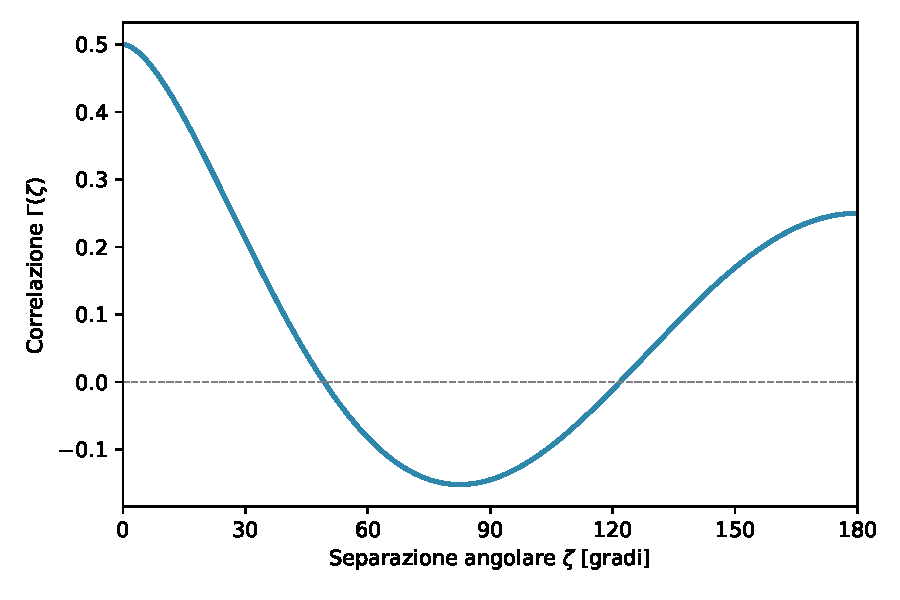
\includegraphics[width=0.7\textwidth]{Figure/cap2/hellings_downs.pdf}
    \caption{\footnotesize Correlazione di Hellings e Downs [Eq.~\eqref{eq:HD}] tra i residui di due pulsar in funzione della loro separazione angolare $\zeta$, per un fondo di onde gravitazionali isotropo e non polarizzato.}
    \label{fig:HD}
\end{figure}

Per il segnale nella singola pulsar (la ``autocorrelazione'') conta invece solo lo spettro: mediando la risposta~\eqref{eq:redshift_GW} sulle direzioni di provenienza e passando dal redshift al residuo tramite la~\eqref{eq:residuo_GW}, che in frequenza corrisponde a dividere per $(2\pi f)^2$ lo spettro di potenza, si ottiene esattamente la densità spettrale~\eqref{eq:psd_gwb}, $S_{\mathrm{GWB}}(f) = h_c^2/(12\pi^2 f^3)$~\cite{Taylor2021}. È questa la componente del GWB che compare nell'analisi di una singola pulsar come quella svolta in questa tesi.

%%%%%%%%%%%%%%%%%%%%%%%%%%%%%%%%%%%%%%%%%%%%%%%%%%%%%%%%%%%%%%%%%%%%%%%%%%%%%%%%%%%%%%%%%%
\section{I Pulsar Timing Array oggi} \label{sec:PTA_oggi}

Esistono diverse collaborazioni PTA nel mondo: l'europea EPTA, che collabora con l'indiana InPTA; la nordamericana NANOGrav; l'australiana PPTA; la cinese CPTA e, più recentemente, MeerKAT PTA in Sudafrica. Dati e analisi vengono condivisi nell'ambito dell'\textit{International Pulsar Timing Array} (IPTA)~\cite{Shaifullah2025}.

Nel giugno 2023 diverse collaborazioni hanno pubblicato in modo coordinato i risultati delle proprie analisi~\cite{EPTA2023_GWB, NANOGrav2023, PPTA2023, CPTA2023}. Tutte hanno trovato un processo rosso comune a tutte le pulsar, con ampiezza di qualche $10^{-15}$ per $\gammagwb = 13/3$, compatibile con le previsioni per una popolazione di SMBHB, e indicazioni della correlazione di Hellings e Downs con una significatività che varia da un dataset all'altro, nei casi migliori di circa $3$--$4\sigma$. % TODO: controllare i numeri esatti nei singoli paper
Per l'EPTA DR2, che comprende 25 MSP osservate da sei radiotelescopi europei su un arco temporale fino a circa 25 anni, l'evidenza più forte emerge nel sottoinsieme dei dati più recenti, acquisiti con strumentazione di nuova generazione (\textit{DR2new}); lasciando libero l'indice spettrale, l'analisi di questo sottoinsieme favorisce $\log_{10}\Agwb \simeq -14$ e $\gammagwb \simeq 2.7$~\cite{EPTA2023_GWB}. % TODO: verificare valori (log10A = -13.94, gamma = 2.71?)

Non si tratta ancora di una rivelazione definitiva, convenzionalmente associata a una significatività di $5\sigma$, e l'interpretazione astrofisica del segnale (incluso il valore di $\gammagwb$, che sembra preferire valori inferiori a $13/3$) è ancora oggetto di studio. Un ruolo centrale in questo dibattito è giocato dalla modellizzazione del rumore delle singole pulsar~\cite{EPTA2023_noise, Ferranti2025}: poiché il segnale gravitazionale e diverse componenti di rumore hanno la stessa forma spettrale a legge di potenza, una descrizione inadeguata del rumore può assorbire parte del segnale o, al contrario, simularlo. Le possibili \textit{degenerazioni} tra i parametri del modello di rumore di una pulsar, e tra questi e un eventuale GWB, sono l'oggetto di questa tesi.

%========================================================================================
%  CAPITOLO 3 — IL MODELLO DI RUMORE DI UNA PULSAR
%  Obiettivo: descrivere tutte le componenti del modello usato nelle analisi.
%  Lunghezza indicativa: 5-6 pagine.
%  Fonti: Taylor (2021) cap. 7, Shaifullah (2025) sez. 3, EPTA DR2 paper II (EPTA2023_noise),
%         Lentati et al. (2016), tesi di Irene sez. 2.1.
%========================================================================================

\chapter{Il modello di rumore di una pulsar} \label{chpt:rumore}
\sloppy

% Intro: i residui = segnale + rumore; il rumore si divide in bianco e rosso; il rosso si
% divide in acromatico e cromatico. Tabella riassuntiva dei 6 parametri usati in tesi.

\section{Rumore bianco} \label{sec:rumore_bianco}
% - Incertezza radiometrica sui TOA, jitter.
% - Parametri per backend: EFAC (riscala le barre d'errore), EQUAD/TNEQUAD (aggiunge in
%   quadratura), ECORR (correlato tra TOA della stessa osservazione).
% - Formula: sigma^2 = EFAC^2 * (sigma_TOA^2 + EQUAD^2).
% - Nella tesi: fissati ai valori del noisedict (marginalizzati separatamente).

\section{Rumore rosso acromatico} \label{sec:rumore_rosso}
% - Spin noise: irregolarità della rotazione. Non dipende dalla frequenza radio.
% - Legge di potenza P(f) = A^2/(12 pi^2) (f/fyr)^(-gamma) fyr^(-3)
%   -> stessa forma del GWB (Eq. psd_gwb)! Parametri: red_noise_log10_A, red_noise_gamma.

\section{Rumore cromatico: dispersione e scattering} \label{sec:rumore_cromatico}
% - Variazioni di DM nel tempo (moto relativo pulsar-Terra-ISM): ritardo prop. a nu^-2.
%   Parametri: dm_gp_log10_A, dm_gp_gamma.
% - Scattering nel mezzo interstellare: ritardo prop. a nu^-alpha, alpha = 4 (spettro di
%   Kolmogorov darebbe 4.4). Parametri: sv_gp_log10_A, sv_gp_gamma (+ sv_gp_alpha se libero).
% - Perché serve una buona copertura in frequenza radio (Ferranti2025).

\section{Processi gaussiani e base di Fourier} \label{sec:GP}
% - Ogni processo rosso scritto come somma di seni e coseni alle frequenze k/T,
%   k = 1..N, con coefficienti gaussiani di varianza data dalla PSD.
% - Per i processi cromatici la base è moltiplicata per (nu/nu_ref)^(-alpha).
% - Numero di componenti di Fourier per J1640+2224 (dal noisedict di DR2low).
% - Figura: PSD delle tre componenti + white noise per J1640 (stile Irene fig. 2.7).

\section{Riepilogo del modello} \label{sec:riepilogo_modello}
% Tabella: componente | dipendenza da nu | parametri | prior.

%========================================================================================
%  CAPITOLO 4 — INFERENZA BAYESIANA E STRUMENTI DI ANALISI
%  Lunghezza indicativa: 5-6 pagine.
%  Fonti: Thrane & Talbot (2019), Taylor (2021) cap. 5-7, tesi di Irene cap. 3 (impostazione).
%========================================================================================

\chapter{Inferenza bayesiana e strumenti di analisi} \label{chpt:inferenza}
\sloppy

\section{Teorema di Bayes, likelihood e prior} \label{sec:bayes}
% - Posterior = likelihood x prior / evidenza. Marginalizzazione. Intervalli di credibilità.

\section{La likelihood per il pulsar timing} \label{sec:likelihood_PTA}
% - Residui gaussiani: r = M eps + F a + n.
% - Likelihood marginalizzata sui coefficienti: ln L = -1/2 r^T C^-1 r - 1/2 ln det(2 pi C),
%   C = N + T B T^T (formula di Woodbury per l'inversione).

\section{Campionamento: Markov Chain Monte Carlo} \label{sec:MCMC}
% - Metropolis-Hastings, PTMCMC (parallel tempering, salti adattivi).
% - Impostazioni usate: Niter = 1e6, thin = 10, burn-in 25%, ~1e5 campioni.
% - Convergenza: tempo di autocorrelazione (emcee), corner plot.

\section{Enterprise e Discovery} \label{sec:enterprise_discovery}
% - Enterprise: standard della comunità (Python/NumPy).
% - Discovery: nuova implementazione in JAX, differenziabile, GPU, compilazione JIT.
% - Perché è importante validarla -> capitolo 5.
% - Workstation di dipartimento (GPU) per i run lunghi.

%========================================================================================
%  CAPITOLO 5 — VALIDAZIONE DI DISCOVERY SU PSR J1640+2224
%  Lunghezza indicativa: 5-6 pagine.
%  Notebook: 01_DR2low_Discovery_vs_Enterprise, 02_DR2newplus, 03_Simulazioni_seed.
%========================================================================================

\chapter{Validazione di Discovery su PSR J1640+2224} \label{chpt:validazione}
\sloppy

\section{Dati: EPTA DR2low e DR2new+} \label{sec:dati}
% - J1640+2224: numero di TOA, arco temporale, backend, bande radio.

\section{Confronto tra Discovery ed Enterprise} \label{sec:confronto_disc_ent}
% - Stesso modello a 6 parametri, stessi prior.
% - Figura candidata: corner_confronto_NEW.png (Discovery blu #2E86AB, Enterprise rosso #C73E1D).
% - Tabella mediane e intervalli al 68%. Bimodalità nel red noise.

\section{DR2low e DR2new+} \label{sec:dr2low_dr2new}
% - Figure candidate: corner_DR2low_vs_DR2new.png, corner_DR2low_vs_DR2new_DM.png.

\section{Test su dati simulati} \label{sec:test_simulati}
% - Simulazioni con i valori veri noti, recovery.
% - Test con semi diversi (seed 1, 17, 42): il seed 1 non è patologico.
% - Figure candidate: corner_recovery_sim.png, corner_sim_seed17_vs_seed1.png, corner_reali_vs_simulati.png.

%========================================================================================
%  CAPITOLO 6 — STUDIO DELLE DEGENERAZIONI  (il cuore della tesi)
%  Lunghezza indicativa: 8-10 pagine.
%  Notebook: 04-14, Simulations*.ipynb.
%========================================================================================

\chapter{Studio delle degenerazioni} \label{chpt:degenerazioni}
\sloppy

\section{Iniezione di un fondo di onde gravitazionali} \label{sec:iniezione_GWB}
% - Tre ampiezze log10_A = -14.5, -15.0, -15.5 con gamma = 13/3, analizzate con il modello
%   a 6 parametri SENZA GWB: il GWB viene assorbito dal red noise?
% - Iniezione con i valori di EPTA DR2new (log10_A = -14, gamma = 2.7) e con gamma = 13/3.
% - Figure candidate: corner_gwb_tre_ampiezze_v2.png, corner_senza_vs_gwb_A145_v2.png, ...,
%   corner_sim_gwb_A140_g27.png, corner_reali_vs_GWB_tre_ampiezze.png.
%   (simulati verde #2A9D8F, con GWB viola #6A4C93)

\section{Degenerazione tra dispersione e scattering} \label{sec:DM_SV}
% - La forma a "L" nei piani (dm_gp, sv_gp): presente già senza GWB o introdotta dal GWB?
% - Esperimento con i valori veri di DM e SV scambiati (swap).

\section{L'indice cromatico dello scattering} \label{sec:alpha}
% - Simulazione con alpha = 4.4, analisi con alpha = 4.0 (modello sbagliato) e 4.4 (corretto).
% - alpha lasciato libero (sv_gp_alpha), con e senza GWB.
% - Dati reali con alpha = 4.4.
% - Figure candidate: corner_sim_sv44_errato_vs_corretto.png, corner_sim_sv44_fixed_vs_alphafree.png,
%   corner_sim_sv44_alphafree_degenerazione.png, corner_gwb_A140_sv44_alphafree_degenerazione.png.

\section{Discussione} \label{sec:discussione}

%========================================================================================
%  CONCLUSIONI  (1-2 pagine)
%  Riassunto dei risultati principali + limiti dell'analisi (una sola pulsar) + prospettive
%  (analisi su più pulsar / array completo, più bande radio, ...).
%========================================================================================

\addcontentsline{toc}{chapter}{Conclusioni}
\chapter*{Conclusioni}
\markboth{Conclusioni}{Conclusioni}
\label{Conclusioni}
\sloppy

\TODO{da scrivere alla fine}


%----------------------------------------------------------------------------------------
%	BIBLIOGRAFIA (le voci stanno in references.bib)
%----------------------------------------------------------------------------------------
\bibliographystyle{unsrtnat}   % ordine di citazione, con DOI e link arXiv
\bibliography{references}

% \begin{acknowledgements}
%     ...
% \end{acknowledgements}

\end{document}
